\documentclass[11pt]{article}
\usepackage[T1]{fontenc}
\usepackage{lmodern}
\usepackage[margin=1in]{geometry}
\usepackage{amsmath,amssymb,amsthm,mathtools}
\usepackage{microtype,booktabs,array,graphicx,xcolor}
\usepackage{enumitem}
\usepackage[colorlinks=true,linkcolor=blue!45!black,citecolor=blue!45!black,urlcolor=blue!45!black]{hyperref}
\usepackage[nameinlink,noabbrev]{cleveref}
\usepackage{fancyhdr}
\pagestyle{fancy}
\fancyhf{}
\fancyhead[L]{\small Hidden symplectic forms}
\fancyhead[R]{\small Complete critical law}
\fancyfoot[C]{\thepage}
\setlength{\headheight}{14pt}
\setlength{\emergencystretch}{2em}
\setlist{itemsep=3pt,topsep=5pt}
\newtheorem{theorem}{Theorem}[section]
\newtheorem{lemma}[theorem]{Lemma}
\newtheorem{proposition}[theorem]{Proposition}
\newtheorem{corollary}[theorem]{Corollary}
\theoremstyle{definition}
\newtheorem{definition}[theorem]{Definition}
\theoremstyle{remark}
\newtheorem{remark}[theorem]{Remark}
\newcommand{\F}{\mathbb F_q}
\newcommand{\Alt}{\operatorname{Alt}}
\newcommand{\TV}{d_{\mathrm{TV}}}
\newcommand{\E}{\mathbb E}
\newcommand{\Pbb}{\mathbb P}
\newcommand{\qbinom}[2]{\genfrac{[}{]}{0pt}{}{#1}{#2}_q}
\newcommand{\Bin}{\operatorname{Bin}}
\newcommand{\rank}{\operatorname{rank}}
\newcommand{\GL}{\operatorname{GL}}
\newcommand{\Sp}{\operatorname{Sp}}
\newcommand{\ind}{\mathbf 1}
\title{The complete critical law for hidden symplectic forms\\[5pt]
\large Candidate-space universality, independent singularity patterns,\\
and optimal testing and recovery}
\author{Research prepared for Vladimir Reshetnikov}
\date{27 November 2026}
\hypersetup{pdftitle={The complete critical law for hidden symplectic forms},
 pdfauthor={Research prepared for Vladimir Reshetnikov},
 pdfsubject={Finite-field probability and an unconditional extension of the ProveIt GRH program}}
\begin{document}
\maketitle
\begin{abstract}
The ProveIt symplectic program studies observations of random two-planes
isotropic for one hidden nondegenerate alternating form. Recent reports locate
the recovery threshold at $\binom n2-1$ observations and determine the critical
dimension of the linear candidate space. They leave the optimal test using all
observations open. We determine that complete critical experiment.
At $t=\binom n2-1+a$, the null candidate dimension tends to the classical
rectangular finite-field law $\pi_{a-1}$; conditional on dimension $k$, the
number of compatible nondegenerate projective forms tends to
$\Bin((q^k-1)/(q-1),\omega_q)$, where
$\omega_q=\prod_{j\ge1}(1-q^{-(2j-1)})$.
The planted law is its explicit size bias. This gives exact limiting optimal
testing, Bayes recovery, and unique-candidate recovery probabilities.
The proof establishes two further results: total-variation universality of
the entire candidate subspace for decomposable observations, and joint
asymptotic independence of nonsingularity for every distinct projective
combination of finitely many random alternating matrices.
Dimension-only testing is strictly suboptimal at every fixed offset.
The optimal procedures have polynomial expected running time in the critical
window. All theorems are unconditional and include characteristic two.
\end{abstract}
\vspace{3pt}
\noindent\textbf{Status.} Complete mathematical proofs with exact finite
checks and reproducible computations. No new Lean formalization is claimed.
Novelty is assessed against a pinned repository snapshot and the primary
literature identified in \cref{sec:provenance}.
\tableofcontents
\section{The result and the gap it closes}
\label{sec:main}

The source program has a substantial finite-field strand: spanning estimates,
symplectic frames, compressed observations, and the extent to which partial
linear information reveals an underlying alternating form. The present paper
continues that strand. Its connection to the GRH project is methodological and
explicit; no assertion about zeros of an $L$-function is used in any proof.

The immediate predecessors \cite{hidden,critical} already established the
sample threshold and the distribution of the candidate space's dimension.
The remaining question is more precise: \emph{how many of those linear
candidates are actually nondegenerate, and how much does that information
improve testing and recovery?} Two spaces of the same dimension can have very
different answers. Our main theorem determines this missing distribution.

\subsection{The experiment}

Fix a prime power $q$ and let $n\ge4$ be even. Put
\[
 V=\F^n,\qquad E=\Alt(V),\qquad
 D=\binom n2,\qquad d=D-1.
\]
Here an alternating form is a bilinear form $H$ with $H(v,v)=0$ for every
$v$. This definition also applies in characteristic two. Nondegeneracy means
that $H(v,w)=0$ for every $w$ forces $v=0$. Forms differing by a nonzero scalar
are identified; a projective form is such an equivalence class.

Under the \emph{null law} $Q_{n,t}$ we observe independent uniform
two-dimensional subspaces $\Pi_1,\ldots,\Pi_t$ of $V$.
Under the \emph{planted law} $P_{n,t}$ we first choose a uniform nondegenerate
projective form $[H]$, and then independently choose each $\Pi_i$ uniformly
among the $H$-isotropic two-planes. Thus $H$ is chosen once and is common to
every observation. Define
\begin{align}
 N&=\{G\in E:G|_{\Pi_i\times\Pi_i}=0\text{ for all }i\},
 &K&=\dim N,\label{eq:candidates}\\
 Z&=\#\{[G]\in\mathbb P(N):G\text{ is nondegenerate}\}.
 \label{eq:Z}
\end{align}
The entire space $N$ is found by solving $t$ homogeneous linear equations in
$D$ unknowns. Under the planted law, $Z\ge1$ because $[H]$ is a candidate.

\subsection{The explicit critical distribution}

Use the constants and probability masses
\begin{gather}
 g_j=\prod_{i=1}^j(1-q^{-i}),\qquad
 g_\infty=\prod_{i\ge1}(1-q^{-i}),\qquad
 \omega_q=\prod_{i\ge1}(1-q^{-(2i-1)}),\label{eq:products}\\
 c_q=\frac{\omega_q}{1-q^{-1}},\qquad
 m_k=\frac{q^k-1}{q-1},\qquad
 \lambda_a=c_q q^{-a},\label{eq:constants}\\
 \pi_b(k)=\frac{g_\infty q^{-k(k+b)}}{g_k g_{k+b}}\quad
 (k\ge\max(0,-b)),\label{eq:pi}
\end{gather}
and set $\pi_b(k)=0$ elsewhere. The law $\pi_b$ is the classical limiting
kernel dimension of a uniform $(D+b)\times D$ matrix over $\F$ as
$D\to\infty$ \cite{fulman}. It is not a new marginal distribution.

\begin{theorem}[The complete critical experiment]
\label{thm:main}
Fix $q$ and an integer $a$, and set $t=d+a$. As even $n\to\infty$, the joint
law of $(K,Z)$ converges in total variation as follows.
\begin{enumerate}
\item Under $Q_{n,t}$, draw
\[
 K\sim\pi_{a-1},\qquad Z\mid K=k\sim\Bin(m_k,\omega_q).
 \tag{Q}\label{eq:Q-limit}
\]
In particular $Z=0$ when $K=0$.
\item Under $P_{n,t}$, draw
\[
 J\sim\pi_a,\qquad K=1+J,\qquad
 Z\mid K=k\sim1+\Bin(m_k-1,\omega_q).
 \tag{P}\label{eq:P-limit}
\]
\item If $\mathsf Q_a$ denotes the joint law in \eqref{eq:Q-limit}, the law
in \eqref{eq:P-limit} satisfies
\begin{equation}
 \mathsf P_a(k,z)=\frac{z}{\lambda_a}\mathsf Q_a(k,z).
 \label{eq:sizebias}
\end{equation}
The statistic $Z$ determines the exact finite-sample likelihood ratio, so
these formulas determine the limiting optimum over all tests of the complete
observations.
\end{enumerate}
\end{theorem}

The binomial statement is conditional on a \emph{fixed finite} dimension.
It does not assert finite-$n$ independence, or independence for a number of
forms growing with $n$. The candidate dimension remains random in the limit;
averaging that randomness is essential.

\begin{corollary}[Optimal testing and recovery curves]
\label{cor:curves}
With $(K,Z)\sim\mathsf Q_a$, define
\begin{align}
 T_q(a)&=\frac12\E\left|\frac{Z}{\lambda_a}-1\right|,
 \label{eq:T}\\
 R_q(a)&=\frac1{\lambda_a}
 \sum_{k\ge0}\pi_{a-1}(k)\bigl[1-(1-\omega_q)^{m_k}\bigr],
 \label{eq:R}\\
 U_q(a)&=\sum_{k\ge1}\pi_a(k-1)(1-\omega_q)^{m_k-1}.
 \label{eq:U}
\end{align}
Then $\TV(P_{n,d+a},Q_{n,d+a})\to T_q(a)$; the optimal probability of
recovering the hidden projective form tends to $R_q(a)$; and, under the
planted law, the probability of a unique compatible nondegenerate projective
form tends to $U_q(a)$.
For $a\ge0$, the exact finite-sample optimal test declares the planted law
precisely when $Z>0$, and
\begin{equation}
 T_q(a)=\sum_{k\ge0}\pi_{a-1}(k)(1-\omega_q)^{m_k},\qquad
 R_q(a)=\frac{1-T_q(a)}{\lambda_a}.
 \label{eq:nonnegative}
\end{equation}
The best equal-prior testing success probability tends to $(1+T_q(a))/2$.
\end{corollary}

\subsection{What is gained}

For comparison, the previously known dimension-only testing distance and
linear uniqueness probability are
\begin{align}
 T_q^{\rm dim}(a)&=
 \begin{cases}
 q^{a-1}g_\infty/g_{1-a},&a\le0,\\
 g_\infty/g_{a-1},&a\ge1,
 \end{cases}\label{eq:dimension-curve}\\
 F_q(a)&=\begin{cases}g_\infty/g_a,&a\ge0,\\0,&a<0.\end{cases}
 \label{eq:linear-curve}
\end{align}
We rederive these comparisons below. The new result gives the strict
inequalities
\begin{equation}
 T_q(a)>T_q^{\rm dim}(a),\qquad
 R_q(a)>U_q(a)>F_q(a)\quad(a\in\mathbb Z).
 \label{eq:strict-gain}
\end{equation}
The second inequality is interpreted with $F_q(a)=0$ for negative offsets.
Thus uniqueness among nondegenerate forms can occur even before linear
uniqueness is possible.

For $q=2$ the central offset $a=0$ gives
\[
 T_2(0)=0.411496025791\ldots,\qquad
 T_2^{\rm dim}(0)=0.288788095087\ldots,
\]
and
\[
 R_2(0)=0.701564718009\ldots,\quad
 U_2(0)=0.488389858129\ldots,\quad
 F_2(0)=0.288788095087\ldots.
\]
At $a=-1$, optimal recovery still succeeds with limiting probability
$0.503310957568\ldots$, although a one-dimensional linear candidate space is
impossible. These are limiting probabilities, not finite-size guarantees.

\begin{figure}[htbp]
 \centering
 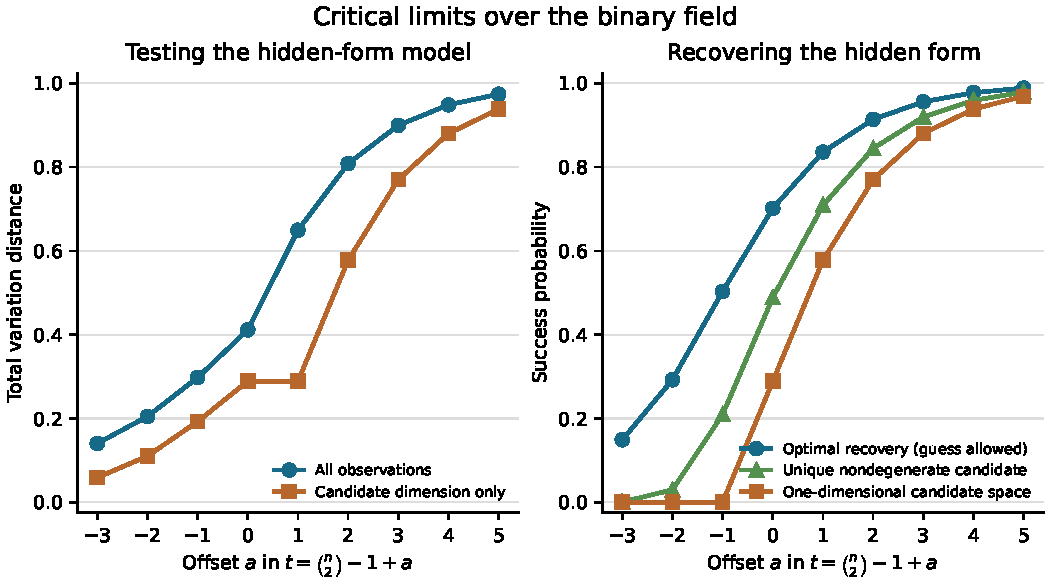
\includegraphics[width=\textwidth]{figures/critical_profiles.pdf}
 \caption{The proved binary-field critical curves. The horizontal variable
 is the integer offset from $d=\binom n2-1$. Lines connect integer evaluations
 for readability; no continuous-offset interpolation is asserted.}
 \label{fig:profiles}
\end{figure}

\subsection{Two independent mathematical advances}

The first new ingredient, \cref{ker:theorem}, replaces the full law of $N$ by
that of the kernel of independent uniform linear equations. Its conclusion
concerns the actual subspace, including its position, and is stronger than a
nullity law. The rows in the observation model are decomposable bivectors,
with extensive dependence among their entries.

The second ingredient, \cref{thm:pencil}, states that the invertibility
indicators of all distinct projective combinations of a fixed family of large
random alternating matrices become independent. As a standalone consequence,
every prescribed pattern of singular and nonsingular projective combinations
has a positive limiting probability. Combining these ingredients with the
exact likelihood gives \cref{thm:main}.

There is also an algorithmic consequence: in the fixed critical window the
exact optimal test and a Bayes optimal recovery rule can be implemented with
$O_{q,a}(n^6)$ expected field operations under either experiment. This is an
expected bound; the candidate enumeration can be exponential on exceptional
inputs. See \cref{prop:algorithm}.

\section{Exact finite-sample structure}
\label{sec:finite}

We include the elementary likelihood calculation from the preceding
hidden-form report \cite{hidden}, because it makes the statistical conclusion
self-contained and specifies exactly which part of the proof is new.

\begin{lemma}[Counts and likelihood]
\label{lem:likelihood}
Let $M_n$ be the number of nondegenerate projective alternating forms on
$\F^n$. Put
\[
 c_n=\prod_{j=2}^{n/2}(1-q^{-(2j-1)}),\qquad
 p_n=\frac{q^{n-2}-1}{q^{n-1}-1}.
\]
Then
\begin{equation}
 M_n=q^{D-1}c_n,\qquad
 \frac{dP_{n,t}}{dQ_{n,t}}=\frac{Z}{M_np_n^t},\qquad
 \E_Q Z=M_np_n^t.
 \label{eq:finite-likelihood}
\end{equation}
The posterior distribution of $[H]$ under the planted model is uniform on
the $Z$ compatible nondegenerate projective forms. Consequently the exact
Bayes optimal recovery probability is
\begin{equation}
 \operatorname{Rec}_{n,t}=\frac{Q_{n,t}(Z>0)}{M_np_n^t}.
 \label{eq:finite-recovery}
\end{equation}
\end{lemma}

\begin{proof}
The general linear group acts transitively on nondegenerate alternating
forms, with stabilizer $\Sp_n(q)$. Counting ordered bases and symplectic
bases gives
\[
 |\GL_n(q)|=q^{n^2}\prod_{j=1}^n(1-q^{-j}),\qquad
 |\Sp_n(q)|=q^{n(n+1)/2}\prod_{j=1}^{n/2}(1-q^{-2j}).
\]
Their quotient is
$q^D\prod_{j=1}^{n/2}(1-q^{-(2j-1)})$. Dividing by $q-1$ proves the
formula for $M_n$.

For each nonzero $u$, the form $H(u,\cdot)$ is a nonzero linear functional.
Among the $q^n-q$ vectors $v$ independent of $u$, precisely $q^{n-1}-q$
satisfy $H(u,v)=0$. Therefore a uniform two-plane is $H$-isotropic with
probability $p_n$. Every compatible $[H]$ gives likelihood $p_n^{-t}$
relative to $Q$, and incompatible forms give likelihood zero. Averaging over
the $M_n$ forms proves \eqref{eq:finite-likelihood} and the uniform posterior.
Conditional optimal recovery has probability $1/Z$ under $P$, so
\[
 \E_P\frac1Z
 =\E_Q\left[\frac{Z}{M_np_n^t}\frac{\ind_{\{Z>0\}}}{Z}\right]
 =\frac{Q(Z>0)}{M_np_n^t},
\]
where $\ind_{\{Z>0\}}/Z$ is defined to be zero when $Z=0$.
All the basis counts and orthogonality statements are valid in characteristic
two; no division by two is involved.
\end{proof}

The full posterior depends on the observations only through $N$. The
likelihood for testing $P$ against $Q$ depends only on $Z$. The identities of
the candidate forms are still needed to output a recovered form; a bare
count does not encode those identities.

At $t=d+a$,
\begin{equation}
 M_np_n^t=c_nq^{-a}(qp_n)^t\longrightarrow c_qq^{-a}=\lambda_a,
 \label{eq:mean-limit}
\end{equation}
because $qp_n=1-O_q(q^{-n})$ and $t=O(n^2)$. Notice also that
\begin{equation}
 M_np_n^{d+a}<c_nq^{-a}<1\qquad(a\ge0).
 \label{eq:threshold-below-one}
\end{equation}
The likelihood ratio therefore exceeds one exactly when $Z>0$ for every
finite $n\ge4$ at these offsets. What remains to be determined is the
probability of that event and the full law of $Z$.

\section{Universality of the complete candidate subspace}
\label{sec:kernel-universality}

The critical nullity law alone does not determine the optimal test.
Two candidate subspaces of the same dimension can contain different
numbers of nondegenerate forms.  We therefore compare the laws of the
entire candidate subspaces, including their positions in the vector
space of alternating forms.

Throughout this section, $q$ is fixed, $n$ tends to infinity through
even integers,
\[
 E=\Alt(\F^n),\qquad D=\binom n2,\qquad t=D+b,
\]
and $b\in\mathbb Z$ is fixed.  The global offset notation is
$b=a-1$.  Under the null model, $K_1,\ldots,K_t$ are independent
uniform two-dimensional subspaces of $\F^n$, and
\[
 N=\{G\in E:G|_{K_i\times K_i}=0\text{ for every }i\}.
\]
Let $N^{\mathrm u}$ be the common kernel of $t$ independent uniform
linear functionals on $E$.  All total variation distances below
compare probability measures on the full lattice of subspaces of
the same $D$-dimensional space $E$.

\begin{theorem}[Complete kernel universality]
\label{ker:theorem}
For every fixed prime power $q$ and integer $b$,
\[
 \TV\bigl(\mathcal L(N),\mathcal L(N^{\mathrm u})\bigr)
 \longrightarrow0.
\]
Consequently, conditional on any fixed candidate dimension having
positive limiting probability, $N$ is asymptotically uniform on the
corresponding Grassmannian.  The conclusion holds in characteristic
two as well.
\end{theorem}

The proof has two parts.  We first compare, in aggregate, the
probabilities that each fixed-dimensional subspace survives all
observations.  A quantitative truncation of subspace M\"obius
inversion then upgrades those comparisons to total variation.  This
avoids an unproved assertion that a collection of moments uniquely
determines the limiting distribution.

\subsection{Exact subspace survival probabilities}

Write
\[
 \delta_n=(q+1)q^{-n}-q^{1-2n}.
\]
This is the probability that two independent uniform vectors
$u,v\in\F^n$ are linearly dependent.  Fix a nontrivial additive
character $\psi$ of $\F$.  Averaging first over $v$ gives
\begin{equation}
 \E_{u,v}\psi(G(u,v))=q^{-\operatorname{rank}G}
 \qquad(G\in E).
 \label{ker:rank-fourier}
\end{equation}
If $M\le E$ has dimension $j$, character orthogonality therefore
gives, before conditioning on independence,
\[
 \Pbb\{G(u,v)=0\text{ for all }G\in M\}
 =q^{-j}\sum_{G\in M}q^{-\operatorname{rank}G}.
\]
Every alternating form vanishes on a dependent pair.  Conditioning
on independence, which makes $\langle u,v\rangle$ a uniform
two-plane, proves the exact formula
\begin{equation}
 h(M):=\Pbb\{G|_{K\times K}=0\text{ for all }G\in M\}
 =\frac{q^{-j}\displaystyle\sum_{G\in M}
                 q^{-\operatorname{rank}G}-\delta_n}
        {1-\delta_n}.
 \label{ker:survival}
\end{equation}
In particular,
\begin{equation}
 \Pbb(M\le N)=h(M)^t,
 \qquad
 \Pbb(M\le N^{\mathrm u})=q^{-jt}.
 \label{ker:inclusion}
\end{equation}

We use the Gaussian binomial notation
\[
 \qbinom{m}{j}
 =\prod_{i=0}^{j-1}\frac{q^m-q^i}{q^j-q^i},
 \qquad
 g_j=\prod_{i=1}^j(1-q^{-i}),\qquad
 g_\infty=\prod_{i=1}^{\infty}(1-q^{-i}).
\]
As usual, the Gaussian binomial is zero outside $0\le j\le m$.
The empty product is one.

\begin{lemma}[Aggregate inclusion comparison]
\label{ker:aggregate}
For each fixed nonnegative integer $j$,
\begin{equation}
 \Delta_{n,j}:=
 \sum_{\substack{M\le E\\\dim M=j}}
 \left|h(M)^t-q^{-jt}\right|
 \longrightarrow0.
 \label{ker:aggregate-limit}
\end{equation}
For $j\ge1$, $t\ge1$, and any integer $0\le R<n$, define
\begin{align*}
 B_{n,R}&=\#\{G\in E:\operatorname{rank}G\le R\},\\
 \eta_q&=q^{-1}+(1-q^{-1})q^{-2}<1,\\
 A_{n,j,R}&=\frac{\eta_q+q^{j-R}}{1-\delta_n},\\
 \theta_{n,j,R}&=
 \frac{(q^j-1)(q^{-R}+\delta_n)}{1-\delta_n},\\
 m_{n,j}&=\qbinom Dj q^{-jt}.
\end{align*}
Then the following finite bound holds:
\begin{equation}
 \begin{split}
 \Delta_{n,j}\le{}&
 m_{n,j}\bigl(e^{t\theta_{n,j,R}}-1\bigr)\\
 &+A_{n,j,R}^{t}
       \sum_{s=1}^j B_{n,R}^{s}q^{-(j-s)b}
   +\sum_{s=1}^jB_{n,R}^{s}q^{-sD-jb}.
 \end{split}
 \label{ker:finite-aggregate}
\end{equation}
Moreover,
\begin{equation}
 B_{n,R}\le
 g_\infty^{-1}q^{D-\binom{n-R}{2}}
 \le g_\infty^{-1}q^{nR},
 \qquad
 m_{n,j}\le g_j^{-1}q^{-j(j+b)}.
 \label{ker:counts}
\end{equation}
\end{lemma}

\begin{proof}
The case $j=0$ is exact.  For the rank count, the radical of a form
of rank at most $R$ contains an $(n-R)$-space.  There are at most
$g_\infty^{-1}q^{R(n-R)}$ such spaces, and forms vanishing on one
descend to at most $q^{R(R-1)/2}$ alternating forms on its quotient.
This proves the first bound in \eqref{ker:counts}; its second
inequality follows by expanding the exponent.  The bound on
$m_{n,j}$ follows directly from the product formula for the Gaussian
binomial.

For a $j$-space $M$, let $s(M)$ be the dimension of the span of
\[
 \{G\in M:\operatorname{rank}G\le R\}.
\]
If $s(M)=0$, every nonzero element of $M$ has rank greater than $R$.
Equation \eqref{ker:survival} then gives
\[
 \left|\frac{h(M)}{q^{-j}}-1\right|
 \le\theta_{n,j,R}.
\]
For a nonnegative number $x$ with $|x-1|\le\theta$ and a positive
integer $t$, $|x^t-1|\le e^{t\theta}-1$.  Summing over these generic
$M$ gives the first term of \eqref{ker:finite-aggregate}.

Suppose next that $s(M)=s\ge1$.  Its low-rank span has a basis
consisting of low-rank forms.  Choose an ordered such basis, then
complete it by $j-s$ arbitrary vectors of $E$.  This overcounts the
possible $M$, and gives the upper bound
\begin{equation}
 \#\{M:\dim M=j,\ s(M)=s\}
 \le B_{n,R}^{s}q^{(j-s)D}.
 \label{ker:bad-count}
\end{equation}
Every nonzero alternating form has rank at least two.  All the
low-rank elements of $M$ lie in its specified $s$-space, so
\begin{align*}
 \sum_{G\in M}q^{-\operatorname{rank}G}
 &\le1+(q^s-1)q^{-2}+(q^j-q^s)q^{-R}\\
 &=q^s\bigl(q^{-s}+(1-q^{-s})q^{-2}\bigr)
      +(q^j-q^s)q^{-R}.
\end{align*}
The expression in parentheses is at most $\eta_q$.  Dropping the
negative term in the numerator of \eqref{ker:survival} therefore
shows that
\[
 h(M)\le q^{s-j}A_{n,j,R}.
\]
Together with \eqref{ker:bad-count}, this bounds the sum of
$h(M)^t$ over exceptional spaces by the second term of
\eqref{ker:finite-aggregate}.  Their $q^{-jt}$ contribution is bounded
by the third term.

Finally choose $\sigma$ with $\eta_q<\sigma<1$, put
$\beta=-\log_q\sigma>0$, and set
\[
 R=\left\lfloor\frac{\beta n}{8j}\right\rfloor.
\]
For all sufficiently large $n$, $A_{n,j,R}\le\sigma$ and
$t\theta_{n,j,R}\to0$.  For $1\le s\le j$, the exponent in the
second term satisfies
\[
 snR-\beta t
 \le\frac{\beta n^2}{8}
      -\beta\left(\binom n2+b\right),
\]
which tends to $-\infty$ quadratically.  The third term also tends
to zero quadratically.  This proves \eqref{ker:aggregate-limit}.
For fixed $q,j,b$, the first term is
$O_{q,j,b}(n^2q^{-\beta n/(8j)})$.
\end{proof}

The classification by the \emph{span} of low-rank elements is useful
here.  A small probability that any low-rank form survives does not,
by itself, control high moments of the number of surviving subspaces.
The aggregate estimate does provide that control.

\subsection{A quantitative inversion on the subspace lattice}

For a probability measure $\lambda$ on subspaces of $E$, put
$p_\lambda(M)=\Pbb_\lambda(M\le N)$.  For an integer $K\ge1$, define
the signed measure
\begin{equation}
 I_K(\lambda)(S)=
 \sum_{\substack{M\ge S\\\dim M\le K}}
 (-1)^{\dim M-\dim S}
 q^{\binom{\dim M-\dim S}{2}}p_\lambda(M)
 \quad(\dim S\le K),
 \label{ker:truncated-inversion}
\end{equation}
and set it to zero when $\dim S>K$.  Write $\|\cdot\|_1$ for the
sum of absolute masses, so that total variation between probabilities
is half this norm.

\begin{lemma}[Truncation bound]
\label{ker:inversion-bound}
Let
\[
 C_K=\prod_{i=1}^K(1+q^i).
\]
For every probability measure $\lambda$ on subspaces,
\begin{equation}
 \|\lambda-I_K(\lambda)\|_1
 \le C_K\E_\lambda\qbinom{\dim N}{K}
       +\Pbb_\lambda(\dim N>K).
 \label{ker:truncation-bound}
\end{equation}
For two such measures $\lambda,\lambda'$,
\begin{equation}
 \begin{split}
 \|I_K(\lambda)-I_K(\lambda')\|_1
 \le\sum_{j=0}^K c_j
 \sum_{\substack{M\le E\\\dim M=j}}
 |p_\lambda(M)-p_{\lambda'}(M)|,
 \end{split}
 \label{ker:inversion-comparison}
\end{equation}
where $c_j=\prod_{i=0}^{j-1}(1+q^i)$ and $c_0=1$.
\end{lemma}

\begin{proof}
For integers $r>0$ and $0\le L<r$, the finite $q$-binomial identity
\begin{equation}
 \sum_{j=0}^L(-1)^j q^{\binom j2}\qbinom rj
 =(-1)^Lq^{L(L+1)/2}\qbinom{r-1}{L}
 \label{ker:q-partial}
\end{equation}
follows by induction from the Gaussian-binomial recurrence.
For $L\ge r>0$, the corresponding full sum is zero; for $r=0$ it
is one.

Apply this identity to a deterministic $N$ of dimension $h$.  If
$h\le K$, \eqref{ker:truncated-inversion} reconstructs its point mass
exactly.  If $h>K$, the absolute mass at a subspace $S\le N$ of
dimension $s\le K$ is
\[
 q^{(K-s)(K-s+1)/2}\qbinom{h-s-1}{K-s}.
\]
Using
\[
 \qbinom hs\qbinom{h-s-1}{K-s}
 \le\qbinom hK\qbinom Ks
\]
and summing over $s$ bounds its total mass by
\[
 \qbinom hK
 \sum_{s=0}^K\qbinom Ks q^{(K-s)(K-s+1)/2}
 =\qbinom hK C_K.
\]
The equality is the finite $q$-binomial theorem.  The original point
mass, which lies above dimension $K$, contributes one more to the
error.  Averaging over $N$ proves \eqref{ker:truncation-bound}.

For \eqref{ker:inversion-comparison}, apply the triangle inequality
to \eqref{ker:truncated-inversion} and then interchange its sums.
A fixed $j$-space $M$ contributes the coefficient
\[
 \sum_{s=0}^j\qbinom js q^{\binom{j-s}{2}}
 =\prod_{i=0}^{j-1}(1+q^i)=c_j,
\]
again by the $q$-binomial theorem.
\end{proof}

\begin{proof}[Proof of Theorem~\ref{ker:theorem}]
Let $\mu_n=\mathcal L(N)$ and $\nu_n=\mathcal L(N^{\mathrm u})$.
Counting $K$-subspaces inside the random kernel gives
\[
 \E_{\nu_n}\qbinom{\dim N}{K}
 =\qbinom DK q^{-Kt}
 \longrightarrow
 m_K:=\frac{q^{-K(K+b)}}{g_K}.
\]
Lemma~\ref{ker:aggregate} implies that the corresponding expectation
under $\mu_n$ has the same limit.  Also,
\[
 \Pbb_\lambda(\dim N>K)
 \le\E_\lambda\qbinom{\dim N}{K}
\]
for either measure.  Lemma~\ref{ker:inversion-bound} and
\eqref{ker:aggregate-limit} now give, for each fixed $K\ge1$,
\begin{equation}
 \limsup_{n\to\infty}\|\mu_n-\nu_n\|_1
 \le2(C_K+1)m_K.
 \label{ker:limsup}
\end{equation}
Since $g_K\ge g_\infty>0$ and
\[
 C_K=q^{K(K+1)/2}\prod_{i=1}^K(1+q^{-i}),
\]
we have
\[
 C_Km_K
 =O_q\bigl(q^{-K(K-1)/2-Kb}\bigr)\longrightarrow0.
\]
Let $K\to\infty$ in \eqref{ker:limsup}.  This proves total variation
convergence.  The conditional assertion follows because $N^{\mathrm u}$
is exactly uniform among subspaces of a specified dimension and
conditioning on events with limiting probability bounded away from
zero preserves total variation convergence.
\end{proof}

\begin{corollary}[A finite computable comparison]
\label{ker:finite-TV}
For every $1\le K\le D$ and $t=D+b\ge1$,
\begin{equation}
 \begin{split}
 \TV(\mu_n,\nu_n)\le{}&
 \frac12\sum_{j=0}^Kc_j\Delta_{n,j}
 +(C_K+1)m_{n,K}
 +\frac{C_K+1}{2}\Delta_{n,K}.
 \end{split}
 \label{ker:finite-TV-bound}
\end{equation}
Here $m_{n,K}=\qbinom DK q^{-Kt}$, and the other quantities are
defined in Lemmas~\ref{ker:aggregate} and~\ref{ker:inversion-bound}.
Replacing every $\Delta_{n,j}$ by \eqref{ker:finite-aggregate}, with
an independently chosen integer $R_j\in[0,n-1]$ and the count bound
\eqref{ker:counts}, gives an entirely explicit upper bound.  It may
always be capped at one.  This is a certified computable comparison;
no numerical optimality of its constants is asserted.
\end{corollary}

\begin{proof}
The two Gaussian-binomial moments of order $K$ differ by at most
$\Delta_{n,K}$, and the uniform-row moment is exactly $m_{n,K}$.
Apply \eqref{ker:truncation-bound} to both measures, bound each tail
probability by its order-$K$ moment, and use
\eqref{ker:inversion-comparison}.  Dividing the resulting $\ell^1$
bound by two proves \eqref{ker:finite-TV-bound}.
\end{proof}

\subsection{Transfer of the planted experiment}

Let $Z(S)$ be the number of nondegenerate projective alternating forms
in $S$, and let $M_n$ denote the number of such forms in $E$.
If $H$ is any fixed nondegenerate form, the fraction of two-planes
isotropic for $H$ is
\begin{equation}
 p_n=\frac{q^{n-2}-1}{q^{n-1}-1}.
 \label{ker:isotropic-probability}
\end{equation}
For example, after choosing $u\ne0$, there are $q^{n-1}-q$
independent choices of $v$ with $H(u,v)=0$, out of $q^n-q$
independent choices in total.

In the planted experiment, a uniformly chosen nondegenerate
projective $H$ is shared by all observations, each of which is
uniformly $H$-isotropic.  Its likelihood ratio against the null is
exactly
\begin{equation}
 L_n(N)=\frac{Z(N)}{M_np_n^t}.
 \label{ker:actual-likelihood}
\end{equation}
Thus the entire candidate subspace is a sufficient statistic for
testing and for Bayesian recovery of the form.  Indeed, the
likelihood for each individual $H$ is $p_n^{-t}$ when $H\in N$ and
zero otherwise.  The posterior on the compatible nondegenerate
projective forms is therefore uniform.

There is a corresponding planted uniform-row experiment: choose
the same prior on $H$, then sample uniform linear functionals
annihilating $H$.  Its kernel likelihood against $\nu_n$ is
\begin{equation}
 L_n^{\mathrm u}(N)=\frac{Z(N)}{M_nq^{-t}}.
 \label{ker:uniform-likelihood}
\end{equation}

\begin{proposition}[Universality of both statistical laws]
\label{ker:planted-transfer}
The total variation distance between the two planted kernel laws
also tends to zero.  More strongly,
\begin{equation}
 \sum_{S\le E}Z(S)|\mu_n(S)-\nu_n(S)|\longrightarrow0.
 \label{ker:weighted-TV}
\end{equation}
Consequently the full null/planted pair of candidate-space laws is
asymptotically equivalent to the uniform-linear-constraint pair.
\end{proposition}

\begin{proof}
Put $h=\dim N$.  The elementary formulas
\[
 \qbinom h1=\frac{q^h-1}{q-1},\qquad
 \qbinom h2=\frac{(q^h-1)(q^h-q)}{(q^2-1)(q^2-q)}
\]
and Lemma~\ref{ker:aggregate}, with $j=1,2$, imply
\[
 \sup_n\bigl(\E_{\mu_n}q^{2h}+\E_{\nu_n}q^{2h}\bigr)<\infty
\]
after omission of finitely many initial $n$.  Since
$Z(S)\le(q^{\dim S}-1)/(q-1)$, the contribution to
\eqref{ker:weighted-TV} from $h>K$ is $O_{q,b}(q^{-K})$ uniformly
in $n$.  On $h\le K$ it is at most
$q^K\|\mu_n-\nu_n\|_1/(q-1)$, which tends to zero by
Theorem~\ref{ker:theorem}.  First taking $n\to\infty$, then
$K\to\infty$, proves \eqref{ker:weighted-TV}.

Finally $(qp_n)^t\to1$ because $t=O(n^2)$ and
$qp_n=1+O_q(q^{-n})$.  The elementary count of nondegenerate alternating
forms gives
\[
 M_nq^{-t}=\frac{q^{-b}}{q-1}
     \prod_{i=1}^{n/2}(1-q^{-(2i-1)}),
\]
which has a finite strictly positive limit at the fixed offset $b$.
Comparing the two densities
\eqref{ker:actual-likelihood}--\eqref{ker:uniform-likelihood}, using
\eqref{ker:weighted-TV} and the convergent normalizations, proves
the planted assertion.
\end{proof}


\section{Independent singularity patterns in random alternating spaces}
\label{sec:alternating}

This section proves the second main ingredient without referring to the
observation model. Its content is joint independence across linearly related
matrices; the one-matrix rank law is classical \cite{fulman,pott}.

\begin{theorem}[Projective independence of nonsingularity]
\label{thm:pencil}
Fix $q$, $k$, and pairwise distinct projective points
$[\alpha_1],\ldots,[\alpha_\ell]\in\mathbb P(\F^k)$. Let
$A_1,\ldots,A_k$ be independent uniform alternating $n\times n$ matrices,
where $n$ tends to infinity through even integers. Set
\[
 B_i=\sum_{j=1}^k\alpha_{ij}A_j,\qquad
 I_i=\ind_{\{B_i\text{ is nonsingular}\}}.
\]
Then $(I_1,\ldots,I_\ell)$ converges in total variation to $\ell$ independent
Bernoulli variables with parameter $\omega_q$.
\end{theorem}

\begin{corollary}[The complete pattern and the binomial law]
\label{cor:random-space}
Let $S_n$ be a uniform $k$-dimensional subspace of $\Alt(\F^n)$, with
$q,k$ fixed. The number of nondegenerate projective forms in $S_n$ converges
in total variation to $\Bin(m_k,\omega_q)$. In coordinates given by a uniform
ordered basis, every fixed subset $T\subseteq\mathbb P(\F^k)$ satisfies
\begin{equation}
 \Pbb\{\text{the nonsingular projective combinations are exactly }T\}
 \longrightarrow \omega_q^{|T|}(1-\omega_q)^{m_k-|T|}.
 \label{eq:pattern}
\end{equation}
In particular every such pattern occurs for all sufficiently large even
$n$. The proportion of $k$-dimensional alternating matrix spaces in which
every nonzero matrix is nonsingular tends to $\omega_q^{m_k}$.
\end{corollary}

\subsection{A tensor-rank rigidity lemma}

\begin{lemma}[Equality forces a direct sum]
\label{lem:tensor}
Let $U_1,\ldots,U_\ell$ be subspaces of a finite-dimensional vector space
$V$ over $\F$, and let $\alpha_i\in\F^k$ be nonzero and pairwise
nonproportional. Define
\[
 U=\sum_iU_i,\qquad W=\sum_i\alpha_i\otimes U_i\subseteq\F^k\otimes V.
\]
Then $\dim W\ge\dim U$, with equality if and only if
$U=\bigoplus_iU_i$.
\end{lemma}

\begin{proof}
Extend scalars to an infinite field containing $\F$. Tensor ranks,
dimensions, and the direct-sum property are unchanged. Choose a linear
functional $f$ on the coefficient space with $f(\alpha_i)\ne0$ for every
$i$. Contraction $C_f=f\otimes\mathrm{id}$ maps $W$ onto $U$, so
$\dim W\ge\dim U$.

If equality holds, this contraction is an isomorphism. Because the
$\alpha_i$ are pairwise nonproportional, a second functional $g$ can be
chosen such that the ratios $g(\alpha_i)/f(\alpha_i)$ are all distinct:
each forbidden equality is a proper linear hyperplane in the space of
functionals, and finitely many proper hyperplanes do not cover an infinite
vector space. The endomorphism $C_gC_f^{-1}$ of $U$ acts on $U_i$ by the
scalar $g(\alpha_i)/f(\alpha_i)$. Eigenspaces for distinct eigenvalues
have a direct sum, proving the forward implication. Conversely, if the
$U_i$ have a direct sum, then the subspaces $\alpha_i\otimes U_i$ also
have a direct sum of the same total dimension.
\end{proof}

\subsection{Mixed kernel-subspace moments}

Let $\nu_i=\dim\ker B_i$. For fixed nonnegative integers
$r_1,\ldots,r_\ell$, put $r=\sum_i r_i$.

\begin{lemma}[Factorization of all fixed mixed moments]
\label{lem:mixed}
As $n\to\infty$ through even integers,
\begin{equation}
 \E\prod_{i=1}^\ell\qbinom{\nu_i}{r_i}
 \longrightarrow
 \prod_{i=1}^\ell\frac{q^{-r_i(r_i-1)/2}}{g_{r_i}}.
 \label{eq:mixed-moments}
\end{equation}
The contribution from tuples of kernel subspaces not forming a direct sum
is $O_{q,k,\ell,\boldsymbol r}(q^{-n})$.
\end{lemma}

\begin{proof}
Expand the product as a sum over subspaces $U_i\le V$ with
$\dim U_i=r_i$, asking for the probability that $U_i\le\ker B_i$
for all $i$.

First suppose the $U_i$ form a direct sum $U$ of dimension $r$. Choose a
basis adapted to these subspaces and a complement. Because the matrices
$A_j$ are uniform alternating matrices, a common change of basis preserves
their independent uniform distribution. Each matrix entry associated to an
unordered pair of distinct basis vectors is a uniform independent vector
of $\F^k$ across the $k$ matrices.
For a pair with one endpoint in $U_i$ and the other in the complement there
is one equation, with coefficient vector $\alpha_i$. For a pair inside
$U_i$ there is one equation. For a pair with endpoints in distinct $U_i,U_j$
there are two independent equations, since $\alpha_i,\alpha_j$ are linearly
independent. Thus the total constraint codimension is exactly
\begin{align}
 r(n-r)+\sum_i\binom{r_i}{2}+2\sum_{i<j}r_ir_j
 &=\sum_i\left(nr_i-\frac{r_i(r_i+1)}2\right).
 \label{eq:direct-codim}
\end{align}
The probability is $q$ to the negative of this number. A tuple of
independent uniform $r_i$-subspaces forms a direct sum with probability
$1-O_{\boldsymbol r,q}(q^{-n})$. This follows, for example, by a union bound
over nonzero vectors in the intersections with the preceding span; that
span has bounded dimension. Therefore the number of direct-sum tuples is
\[
 (1+O(q^{-n}))\prod_i\qbinom n{r_i}.
\]
Multiplying by the constraint probability and using
$\qbinom n{s}=q^{s(n-s)}(1+o(1))/g_s$ gives the right side of
\eqref{eq:mixed-moments}.

For the remaining tuples write $s=\dim\sum_iU_i<r$ and
$w=\dim\sum_i\alpha_i\otimes U_i$. By \cref{lem:tensor}, $w\ge s+1$.
There are $O_{q,\boldsymbol r}(q^{s(n-s)})$ choices for the tuple: choose
its $s$-dimensional span and then a bounded number of subspace configurations
inside that span. The equations obtained by pairing against a fixed basis
vector outside the span have rank $w$. Different outside basis vectors use
disjoint random entries, so these equations alone impose codimension
$(n-s)w$. Hence the total contribution of such tuples is at most a constant
times
\[
 q^{s(n-s)}q^{-(n-s)w}
 \le q^{-(n-s)}=O(q^{-n}).
\]
There are only finitely many possible values of $s$ for the fixed
$\boldsymbol r$, completing the proof.
\end{proof}

The expressions $\qbinom{\nu}{r}$ are polynomials of degree $r$ in
$x=q^\nu$, with nonzero leading coefficient:
\[
 \qbinom{\nu}{r}=
 \prod_{j=0}^{r-1}\frac{x-q^j}{q^r-q^j}.
\]
They form a basis for polynomials in $x$. Consequently
\cref{lem:mixed} gives factorization in the limit for any fixed product of
polynomials in the $q^{\nu_i}$. That observation alone would not justify
convergence of the nonsingularity indicators. The next step supplies the
needed approximation and uses the even parity of every $\nu_i$.

\subsection{Even-nullity interpolation}

\begin{lemma}[One-matrix law and a uniform tail bound]
\label{lem:alternating-marginal}
Let $A$ be uniform alternating of even order $n$. If $s$ is even and
$0\le s\le n$, then
\begin{equation}
 \Pbb(\dim\ker A=s)
 =q^{-s(s-1)/2}\frac{g_n}{g_s e_{(n-s)/2}},\qquad
 e_j=\prod_{i=1}^j(1-q^{-2i}).
 \label{eq:alt-mass}
\end{equation}
It is zero for odd $s$. In particular, for a constant depending only on $q$,
\[
 \Pbb(\dim\ker A=s)\le C_q q^{-s(s-1)/2},
\]
and $\Pbb(A\text{ nonsingular})\to\omega_q$.
\end{lemma}

\begin{proof}
Choose the radical, an $s$-subspace, and choose a nondegenerate alternating
form on the quotient. There are
\[
 \qbinom ns\,
 q^{(n-s)(n-s-1)/2}
 \prod_{j=1}^{(n-s)/2}(1-q^{-(2j-1)})
\]
forms with that radical dimension. Dividing by $q^{n(n-1)/2}$ and cancelling
products proves \eqref{eq:alt-mass}. The denominator is bounded below by
$g_\infty e_\infty>0$, giving the tail bound. At $s=0$ the product is
the finite odd product converging to $\omega_q$.
\end{proof}

For $R\ge1$, define the polynomial
\begin{equation}
 P_R(x)=\prod_{j=1}^R\frac{1-xq^{-2j}}{1-q^{-2j}}.
 \label{eq:interpolation}
\end{equation}
It equals one at $x=1$ and zero at $x=q^2,q^4,\ldots,q^{2R}$.
For even $s\ge2R+2$,
\[
 |P_R(q^s)|\le e_\infty^{-1}q^{Rs-R(R+1)}.
\]
Using \cref{lem:alternating-marginal} and writing $s=2R+2+2h$ gives
\begin{align}
 \sup_{n\text{ even}}
 \E\bigl|P_R(q^{\dim\ker A})-\ind_{\{\ker A=0\}}\bigr|^2
 &\le C_q\sum_{h\ge0}q^{-R-1-3h-2h^2}
 \le C'_q q^{-R}.
 \label{eq:L2-approx}
\end{align}
In particular, the approximation holds uniformly in the matrix order. This
parity-aware bound avoids relying on a generally invalid moment-determinacy
shortcut.

\begin{proof}[Proof of \cref{thm:pencil}]
It suffices to show that for every subset of the $\ell$ indices the
probability that all the corresponding matrices are nonsingular tends to
$\omega_q$ to the size of that subset. Relabel and consider the first $u$
indices. Put $X_i=q^{\nu_i}$ and $I_i=\ind_{\{\nu_i=0\}}$.
For a fixed $R$, expand the difference of products by telescoping and apply
Cauchy--Schwarz to each term:
\begin{align}
 \left|\E\prod_{i=1}^u I_i-\E\prod_{i=1}^uP_R(X_i)\right|
 \le\sum_{i=1}^u
 \bigl(\E|I_i-P_R(X_i)|^2\bigr)^{1/2}
 \left(\E\prod_{j<i}P_R(X_j)^2\right)^{1/2}.
 \label{eq:telescope}
\end{align}
The remaining indicator factors have absolute value at most one and may be
dropped in this bound. By \cref{lem:mixed}, for fixed $R$ the mixed
polynomial expectations factor in the limit $n\to\infty$. The limiting
one-matrix $L^2$ norm of $P_R$ is bounded by $1+O_q(q^{-R/2})$, using
\eqref{eq:L2-approx}. The first factor in each summand is
$O_q(q^{-R/2})$. Thus the limsup of \eqref{eq:telescope} is
$O_{q,u}(q^{-R/2})$.

Also by mixed polynomial factorization,
\[
 \lim_{n\to\infty}\E\prod_{i=1}^uP_R(X_i)
 =\left(\lim_{n\to\infty}\E P_R(q^{\dim\ker A})\right)^u.
\]
The inner limit differs from $\omega_q$ by $O_q(q^{-R/2})$.
Letting $R\to\infty$ proves the desired probability limit.
Inclusion-exclusion recovers each zero-one pattern from these all-one
probabilities. There are finitely many patterns, so convergence is in total
variation.
\end{proof}

\begin{proof}[Proof of \cref{cor:random-space}]
The probability that $k$ independent uniform vectors in the
$D$-dimensional space $E$ are linearly dependent is
\[
 1-\prod_{j=0}^{k-1}(1-q^{j-D})=O_{q,k}(q^{-D}).
\]
Conditional on independence, their span is a uniform $k$-space and they
are a uniform ordered basis. Conditioning therefore changes the law by
$o(1)$. Apply \cref{thm:pencil} to all $m_k$ projective coefficient
points. Every limiting pattern probability in \eqref{eq:pattern} is positive,
which also proves eventual existence.
\end{proof}

\begin{remark}[Relation to matrix-space density questions]
The case of unrestricted two-dimensional matrix spaces has close antecedents
in \cite[Section 6]{gruica}, which proves the limiting probability
$g_\infty^{q+1}$ that every nonzero matrix in such a space is invertible.
That paper also studies alternating codes in a regime with growing field
size. Our statement fixes $q$ and the dimension of an alternating space,
lets its even matrix order grow, and determines every projective singularity
pattern. The underlying density questions and the classical marginal rank
law are established subjects, not new concepts introduced here.
\end{remark}

\section{The complete experiment and its consequences}
\label{sec:critical-law}

\subsection{Uniform kernels and the rectangular reference law}

Let $U$ be a uniform $(D+b)\times D$ matrix. Counting its kernel and then
an injective map from the quotient gives, for
$\max(0,-b)\le k\le D$,
\begin{equation}
 \Pbb(\dim\ker U=k)
 =q^{-k(k+b)}\frac{g_D g_{D+b}}{g_k g_{D-k}g_{k+b}}.
 \label{eq:finite-nullity}
\end{equation}
For other $k$ the probability is zero. For every fixed $k$, this tends to
$\pi_b(k)$. Moreover
\[
 \E q^{\dim\ker U}=1+(q^D-1)q^{-(D+b)},
\]
by counting vectors in the kernel. This bounds the dimension tails and
establishes convergence in total variation, as well as
$\sum_k\pi_b(k)=1$. Conditional on its dimension, the kernel is uniform
over the corresponding Grassmannian, by invariance under $\GL_D(q)$.

We will also use the fixed Gaussian moments
\begin{equation}
 \E_{K\sim\pi_b}\qbinom K r
 =\frac{q^{-r(r+b)}}{g_r}\qquad(r\ge0).
 \label{eq:reference-moments}
\end{equation}
For finite $D$, the left side before passage to the limit is
$\qbinom D r q^{-r(D+b)}$, since each $r$-subspace survives with that
probability. The analogous bound at order $r+1$ ensures uniform
integrability: Gaussian binomials of order $r$ grow at most as $q^{rK}$,
and the order-$r+1$ moment controls that tail. Passing to the limit proves
\eqref{eq:reference-moments}. In particular every fixed exponential
moment $\E q^{rK}$ is finite. The same moments are uniformly bounded for
the actual candidate space, by \cref{ker:aggregate}.

\subsection{Proof of the complete law}

\begin{proof}[Proof of \cref{thm:main}]
Put $b=a-1$. By \cref{ker:theorem}, the actual null candidate space is
within $o(1)$ in total variation of a uniform-row kernel. The latter has
dimension tending to $\pi_b$ and, conditional on dimension $k$, is a
uniform $k$-subspace of $E$. For each fixed $k$, \cref{cor:random-space}
gives $Z\Rightarrow\Bin(m_k,\omega_q)$ in total variation. First truncate
the dimension at a fixed bound, use the finitely many conditional
convergences there, and then let the bound tend to infinity. Tightness of
the dimension proves convergence of $(K,Z)$ to \eqref{eq:Q-limit}.

The exact likelihood is $Z/\lambda_{n,a}$, where
$\lambda_{n,a}=M_np_n^{d+a}\to\lambda_a>0$ by
\eqref{eq:mean-limit}. Since $Z\le m_K$ and
\begin{equation}
 m_K^2=m_K+q(q+1)\qbinom K2,
 \label{eq:second-point-moment}
\end{equation}
the order-one and order-two aggregate inclusion bounds give a uniform
bound on $\E_Q Z^2$. Therefore the size-bias weights are uniformly
integrable. Truncating $Z$ at a fixed bound and using total variation on
the bounded part proves convergence of the planted joint law to
$z\mathsf Q_a(k,z)/\lambda_a$.

The limit has mean
\[
 \E_{\mathsf Q_a}Z
 =\omega_q\E_{\pi_{a-1}}m_K
 =\frac{\omega_qq^{1-a}}{q-1}=\lambda_a.
\]
Thus this size bias is a probability law. Finally,
\begin{equation}
 \frac{m_k\omega_q}{\lambda_a}\pi_{a-1}(k)
 =q^{a-1}(q^k-1)\pi_{a-1}(k)
 =\pi_a(k-1).
 \label{eq:dimension-sizebias}
\end{equation}
Size-biasing a $\Bin(m_k,\omega_q)$ variable yields
$1+\Bin(m_k-1,\omega_q)$, which proves \eqref{eq:P-limit}.
The finite likelihood factorization in \cref{lem:likelihood} establishes
the claim about tests using all observations.
\end{proof}

\subsection{Optimal testing, recovery, and the strict information gain}

\begin{proof}[Proof of \cref{cor:curves}]
The Neyman--Pearson likelihood rule declares the planted law when
$Z>\lambda_{n,a}$; ties may be decided arbitrarily. The exact total
variation is
\[
 \frac12\E_Q\left|Z/\lambda_{n,a}-1\right|.
\]
The joint-law convergence and the second-moment bound just used imply
convergence to \eqref{eq:T}. The exact recovery identity
\eqref{eq:finite-recovery} and convergence of $Q(Z>0)$ give
\eqref{eq:R}. Under the planted limit, conditional on $K=k$, the
probability that $Z=1$ is $(1-\omega_q)^{m_k-1}$, giving
\eqref{eq:U}.

For $a\ge0$, \eqref{eq:threshold-below-one} proves that $Z>0$ is
already the exact finite-sample optimal test. In the limit
$0<\lambda_a<1$. Because $Z$ is integer-valued, the likelihood difference
$Z/\lambda_a-1$ is negative only at $Z=0$. Its expectation is zero,
so half its absolute mean equals $\Pbb_{\mathsf Q_a}(Z=0)$. This is
\eqref{eq:nonnegative}, including its recovery identity.
\end{proof}

\begin{proposition}[Dimension loses information at every fixed offset]
\label{prop:strict}
For every prime power $q$ and every fixed integer $a$,
\[
 T_q(a)>T_q^{\rm dim}(a),\qquad R_q(a)>U_q(a)>F_q(a).
\]
In particular, the nondegeneracy constraint supplies positive-probability
unique recovery at every fixed negative offset, where linear uniqueness
has probability zero.
\end{proposition}

\begin{proof}
By \eqref{eq:dimension-sizebias}, the limiting dimension likelihood is
$q^{a-1}(q^k-1)$. If $a\ge1$, it is below one at $k=0$ and at
least one at every $k\ge1$; hence its total variation is
$\pi_{a-1}(0)=g_\infty/g_{a-1}$. If $a\le0$, the common minimum
dimension is $k_0=1-a$. The dimension likelihood is below one only
there, with deficit $q^{a-1}$. Therefore its total variation is
$q^{a-1}\pi_{a-1}(k_0)=q^{a-1}g_\infty/g_{1-a}$. This proves
\eqref{eq:dimension-curve}.

For strictness, choose any sufficiently large fixed $k$ with
$\pi_{a-1}(k)>0$ and $m_k>\lambda_a$. Conditional on this $k$, the
binomial law gives positive probability both to $Z=0$ and to $Z=m_k$.
Thus the full likelihood minus one has both signs in this conditional
class, and
\[
 \E\bigl[|Z/\lambda_a-1|\mid K=k\bigr]
 >\left|\E[Z/\lambda_a-1\mid K=k]\right|.
\]
Averaging gives the strict testing gain.

Linear uniqueness means $K=1$. Under the planted limiting law its
probability is $\pi_a(0)$, exactly \eqref{eq:linear-curve}. There
is positive planted probability of $K\ge2$ and $Z=1$: choose any
fixed $k\ge2$ in the support and use $0<\omega_q<1$. This proves
$U_q(a)>F_q(a)$, including negative offsets. Finally, on $Z\ge2$
the optimal recovery rule still succeeds with probability $1/Z>0$,
whereas uniqueness fails. That event also has positive limiting
probability, so $R_q(a)>U_q(a)$.
\end{proof}

\subsection{The candidate count is not Poisson}

The earlier critical chi-square calculation identifies only a second
moment. It does not determine the distribution; the new law exhibits a
specific higher-order difference.

\begin{corollary}[Matching variance, different third moment]
\label{cor:not-poisson}
For the null limiting count $Z$,
\begin{align}
 \E Z&=\operatorname{Var}(Z)=\lambda_a,\label{eq:mean-var}\\
 \E\bigl[Z(Z-1)(Z-2)\bigr]
 &=\lambda_a^3+(q-1)\omega_q\lambda_a^2.
 \label{eq:third-factorial}
\end{align}
In particular $Z$ is not Poisson for any fixed $q,a$. The corresponding
limiting chi-square divergence is
\begin{equation}
 \chi^2(\mathsf P_a\Vert\mathsf Q_a)=\lambda_a^{-1}=q^a/c_q.
 \label{eq:chi}
\end{equation}
The finite-experiment chi-square divergence has this same limit.
\end{corollary}

\begin{proof}
Write $M=m_K$. The expected number of ordered linearly independent
projective $r$-tuples in the uniform reference kernel is
\begin{equation}
 \frac{q^{r(1-a)}}{(q-1)^r}.
 \label{eq:independent-points}
\end{equation}
Indeed, the number of such tuples in a $D$-space is
$\prod_{j=0}^{r-1}(q^D-q^j)/(q-1)^r$, and all their points survive
with probability $q^{-rt}$. Pass to the limit; moment control justifies
this equivalently from \eqref{eq:reference-moments}.

Every ordered pair of distinct projective points is independent. Thus
$\E M=q^{1-a}/(q-1)$ and
$\E M(M-1)=q^{2(1-a)}/(q-1)^2$. For an ordered distinct triple,
either it is independent or its third point lies on the projective line
through its first two. In the latter case there are precisely $q-1$
choices for the third point. Therefore
\[
 \E(M)_3=\frac{q^{3(1-a)}}{(q-1)^3}
 +(q-1)\frac{q^{2(1-a)}}{(q-1)^2},
\]
where $(x)_r=x(x-1)\cdots(x-r+1)$. Conditional binomial thinning
multiplies the $r$th factorial moment by $\omega_q^r$. This proves
\eqref{eq:mean-var}--\eqref{eq:third-factorial}. Since
$d\mathsf P_a/d\mathsf Q_a=Z/\lambda_a$, its chi-square divergence
is $\operatorname{Var}(Z)/\lambda_a^2=1/\lambda_a$.
For finite experiments, the uniform bound on a third moment of $Z$,
obtained from aggregate inclusion moments through order three, makes
$Z^2$ uniformly integrable. Thus the second moment and chi-square
divergence converge as well.
\end{proof}

\subsection{An exact optimal algorithm with polynomial expected cost}

\begin{proposition}[Efficient recovery in the critical window]
\label{prop:algorithm}
Fix $q$ and $a$. Given bases for the observed two-planes, the exact
finite-sample Bayes optimal detector and a Bayes optimal hidden-form
recovery rule can be computed with $O_{q,a}(n^6)$ expected field operations
under either $Q_{n,d+a}$ or $P_{n,d+a}$. A rational likelihood comparison
has polynomial bit complexity. The algorithm has no polynomial
worst-case guarantee for candidate enumeration.
\end{proposition}

\begin{proof}
For a basis $(u_i,v_i)$ of $\Pi_i$, its equation is
$u_i^{\mathsf T}Gv_i=0$. Form the $t\times D$ coefficient matrix and
compute a basis $G_1,\ldots,G_K$ of $N$ by Gaussian elimination. This
takes $O(n^6)$ field operations because $t,D=O(n^2)$.

Enumerate the $m_K$ projective coefficient vectors, normalized so that
their first nonzero coordinate is one. Form the corresponding matrices
$\sum_jx_jG_j$ and compute their ranks. This costs at most
$O(m_K(Kn^2+n^3))$ field operations and determines $Z$ and all compatible
nondegenerate forms. Compare $Z$ to $M_np_n^t$ for the optimal test.
Return any compatible nondegenerate form for Bayes optimal recovery;
the posterior on that list is uniform.

The fixed-order aggregate moments imply
$\sup_n\E_Q q^{rK}<\infty$ for every fixed $r$. Under the planted law,
\[
 \E_P f(K)=\frac{\E_Q[Zf(K)]}{M_np_n^t},\qquad
 Z\le m_K\le q^K/(q-1),
\]
and the denominator tends to the positive constant $\lambda_a$.
Consequently the order-three null moment bounds
$\E_Q[m_K(1+K)]$ and $\E_P[m_K(1+K)]$ uniformly. The expected
enumeration cost is $O_{q,a}(n^3)$, dominated by elimination.
The likelihood threshold is a rational number built from powers of
integers of $O_q(n)$ bits raised to $t=O(n^2)$, together with the exact
form count. Its numerator and denominator have $O_{q,a}(n^3)$ bits,
so exact comparison is polynomial-time.
\end{proof}

For $a\ge0$ the detector can stop as soon as it finds a nondegenerate
candidate, since existence is the exact optimal test. To certify that the
candidate is unique, the rest of the projective space must be checked.
The distinction between an optimal guess and a uniqueness certificate is
reflected in the separate curves $R_q$ and $U_q$.

\section{Verification, provenance, and scope}
\label{sec:provenance}

\subsection{Numerical evaluation of the proved limits}

\Cref{tab:binary} records the binary-field profiles, evaluated from the
proved infinite sums. All entries were recomputed at higher precision and
with larger truncations. They are evaluations of theorems, not estimates
from a simulation.

\begin{table}[htbp]
\centering
\small
\setlength{\tabcolsep}{5pt}
\begin{tabular}{rccccc}
\toprule
$a$ & Full TV & Dimension TV & Bayes recovery & Unique form & Linear uniqueness\\
\midrule
$-2$ & .204664582 & .110014512 & .292186807 & .029601132 & 0\\
$-1$ & .297541183 & .192525397 & .503310958 & .209448088 & 0\\
$0$  & .411496026 & .288788095 & .701564718 & .488389858 & .288788095\\
$1$  & .649349926 & .288788095 & .836030787 & .708770120 & .577576190\\
$2$  & .808320018 & .577576190 & .914018723 & .844641387 & .770101587\\
$3$  & .899761224 & .770101587 & .955969600 & .919767552 & .880116099\\
$4$  & .948740304 & .880116099 & .977719658 & .959230432 & .938790506\\
\bottomrule
\end{tabular}
\caption{Limiting probabilities and total variation distances for $q=2$.
Total variation is a testing advantage, not itself a testing success
probability; equal-prior optimal success is $(1+\mathrm{TV})/2$.}
\label{tab:binary}
\end{table}

For completeness, a convenient evaluation formula at negative as well as
nonnegative offsets is obtained by setting
$r=\lceil\lambda_a\rceil-1$ and writing $B_{m,p}(r)$ for the binomial
cumulative probability $\Pbb(\Bin(m,p)\le r)$. Then
\begin{equation}
 T_q(a)=\sum_{k\ge0}\pi_{a-1}(k)
 \left[B_{m_k,\omega_q}(r)
 -\frac{m_k\omega_q}{\lambda_a}B_{m_k-1,\omega_q}(r-1)\right].
 \label{eq:cdf-evaluation}
\end{equation}
For $m_k=0$, the bracket is one, and the second term is set to zero.
The formula also handles a possible integral threshold because a likelihood
tie contributes zero. It follows from
$T_q(a)=\E(1-Z/\lambda_a)_+$ and the elementary truncated-binomial
first-moment identity.

For $L\ge\max(0,-b)$ with $2L+b+1>0$, the tail of the dimension law obeys
\begin{equation}
 \sum_{k\ge L}\pi_b(k)
 \le\frac{q^{-L(L+b)}}{g_\infty(1-q^{-(2L+b+1)})}.
 \label{eq:tail-compute}
\end{equation}
This bounds the omitted tail in \eqref{eq:cdf-evaluation}; for recovery,
multiply the corresponding null-law bound by $1/\lambda_a$.
For a product $\prod_{j\ge1}(1-x_j)$, its omitted relative factor lies
between $1-\sum_{j>J}x_j$ and one whenever that sum is below one.
For $g_\infty$ the sum is $q^{-J}/(q-1)$, and for the odd product
it is $q^{-(2J+1)}/(1-q^{-2})$. Thus product and summation truncation
errors can be bounded explicitly.

The file \texttt{code/critical\_profiles.py} evaluates 39 profiles for
$q=2,3,5$ and $-4\le a\le8$, checks normalization and the first three
factorial moments, strict information gains, and the $a\ge0$ recovery
identity. It uses 90 decimal digits, then repeats the calculation at 120
digits with longer products and dimension cutoffs. The maximum discrepancy
was below $5\times10^{-88}$. Floating-point roundoff is checked by this
repeat; it is not claimed to be a formal interval-arithmetic certificate.

\subsection{Exact finite-field enumeration}

The standard-library program \texttt{code/exact\_binary\_experiment.py}
computes the actual observation experiment on $\mathbb F_2^4$ using
integers and rational arithmetic. There are 35 two-planes and 28
nondegenerate projective alternating forms. Dynamic programming on row
spans represents every ordered sequence of observations without enumerating
the sequences one by one. It checks all sample lengths $0\le t\le10$,
including the $35^{10}=2{,}758{,}547{,}353{,}515{,}625$ sequences at the
largest length. The largest reachable support contains 2,355 row subspaces.

At $n=4,t=5$ the exact values are
\[
 \E_QZ=\frac{972}{2401},\qquad
 \TV(P,Q)=\frac{199008}{300125},\qquad
 \operatorname{Rec}_{4,5}=\frac{101117}{121500}.
\]
The program verifies the likelihood normalization, exact first moment,
dimension coarsening inequality, recovery ordering, and the exact
existence-test identity. These finite-size numbers differ substantially
from their limits; no unjustified small-$n$ accuracy is being asserted.

A second program, \texttt{code/pencil\_checks.py}, exactly enumerates
independent matrix families for
\[
 (q,n,k)=(2,2,2),(2,4,2),(2,4,3),(3,4,2).
\]
It also records seven reproducible simulations of larger families, with
20,000 samples per case and seed 27112026. Exact enumeration and simulation
are labeled separately. For $q=2,n=4,k=2$, the probability that all three
projective combinations are nonsingular is $336/4096$, whereas the product
of the finite marginal probabilities is $(7/16)^3$. For
$q=2,n=4,k=3$, all seven combinations cannot simultaneously be nonsingular,
although their eventual limiting probability is positive. These checks
guard against accidentally claiming finite-size independence. They do not
replace the proof of \cref{thm:pencil}.

\subsection{Repository snapshot and the precise extension}

The examined repository snapshot is
\begin{center}
\texttt{VladimirReshetnikov/ProveIt}\\
\small\texttt{641cd6296144d7c29bcc6569655b473647428b1b}.
\end{center}
Its GRH project describes a merge of 194 reports, with a separate record
of formalized statements. Its declared input is RH and GRH for Dirichlet
$L$-functions, pinned upstream to
\texttt{72fead102f663d5c7a407964a13dc0cf9d977207}. The vendored development
is described there as unmodified and unbuilt \cite{repo}. We did not rerun
its Lean build or independent kernel checks. The present proof has no
dependency on that input theorem.

The directly relevant source branch is the merged article's section
\emph{Spanning, frames, auxiliary characters and matrix statistics},
especially its questions about an unknown source form. The two immediate
incoming predecessors were verified byte-for-byte against their pinned
Git blobs:
\begin{itemize}
\item \texttt{grh\_hidden\_forms\_and\_filters\_2026-11-27.zip},
which proves the additive sample threshold, exact likelihood, Bayes
identity, and critical chi-square limit \cite{hidden}.
\item \texttt{grh\_finite\_observation\_and\_critical\_recovery.zip},
which proves critical dimension universality, dimension-only testing,
linear recovery, and an observation-overhead law \cite{critical}.
\end{itemize}
The second predecessor explicitly leaves the count of compatible
nondegenerate forms and the full-data optimum open. The new contributions
are full subspace universality, the projective singularity-pattern law,
and the resulting complete critical experiment. The old likelihood and
classical marginal rank law are identified as inputs and rederived where
needed, rather than claimed as new results.

\subsection{Literature and limits of the originality claim}

Classical rectangular and alternating rank laws are treated in
Fulman--Goldstein \cite{fulman}. Exact joint rank counts for
$A,B,A+B$ in alternating ensembles are given by Pott--Schmidt--Zhou
\cite{pott}. Structured quadratic-evaluation rows and their rank
thresholds occur in Cascudo--Cramer--Mirandola--Z\'emor \cite{cascudo};
random rank-one tensors and general-position questions are studied by
Randriambololona \cite{randriam}. The rank-metric density work
\cite{gruica} supplies particularly close context for nonsingularity of
every matrix in a random pencil. The current proof combines a different
row ensemble with a full subspace comparison and a fixed-field,
arbitrary-fixed-dimension alternating pattern theorem.

The targeted search and repository comparison did not locate this complete
critical-law result. That supports treating it as a new result of this
investigation relative to the inspected material; it does not establish
worldwide publication priority. The proof has been independently checked
within this task, but has not been externally peer reviewed or formalized
in Lean.

The asymptotic parameters are explicit: $q$, the critical offset $a$, and
the dimension in the standalone pencil theorem are fixed. No uniform
claim is made when these grow with $n$. \Cref{ker:finite-TV} supplies a
computable finite comparison for the kernel step, but the combined
optimal-risk theorem is stated as a limit rather than an optimized
finite-size error estimate. These boundaries do not affect any of the
displayed exact finite identities.

\begin{thebibliography}{10}
\raggedright
\bibitem{repo}
Vladimir Reshetnikov, \emph{ProveIt: Generalized Riemann Hypothesis},
repository snapshot \texttt{641cd6296144d7c29bcc6569655b473647428b1b},
27 November 2026. Project README; Article README; and article sections
\texttt{src.tex} and \texttt{spn.tex}.
\href{https://github.com/VladimirReshetnikov/ProveIt/tree/641cd6296144d7c29bcc6569655b473647428b1b/Analysis/GeneralizedRiemannHypothesis}{Pinned project source}.

\bibitem{hidden}
ProveIt research packet, \emph{Hidden symplectic forms}, 27 November 2026,
in \texttt{grh\_hidden\_forms\_and\_filters\_2026-11-27.zip}.
Git blob \texttt{2af6e2b88464ccb5626c3ec8b8b83d355ff584d2}.
\href{https://github.com/VladimirReshetnikov/ProveIt/blob/641cd6296144d7c29bcc6569655b473647428b1b/Analysis/GeneralizedRiemannHypothesis/docs/incoming/grh_hidden_forms_and_filters_2026-11-27.zip}{Pinned predecessor archive}.

\bibitem{critical}
ProveIt research packet, \emph{Finite observation and critical recovery},
27 November 2026, section ``The complete critical law for linear recovery'',
in \texttt{grh\_finite\_observation\_and\_critical\_recovery.zip}.
Git blob \texttt{edb75dcfadebb64e2ca8e8d53fea54f7f21ed585}.
\href{https://github.com/VladimirReshetnikov/ProveIt/blob/641cd6296144d7c29bcc6569655b473647428b1b/Analysis/GeneralizedRiemannHypothesis/docs/incoming/grh_finite_observation_and_critical_recovery.zip}{Pinned predecessor archive}.

\bibitem{fulman}
Jason Fulman and Larry Goldstein,
\emph{Stein's method and the rank distribution of random matrices over finite
fields}, Annals of Probability \textbf{43} (2015), no.~3, 1274--1314.
\href{https://doi.org/10.1214/13-AOP889}{doi:10.1214/13-AOP889};
\href{https://arxiv.org/abs/1211.0504}{arXiv:1211.0504}.

\bibitem{pott}
Alexander Pott, Kai-Uwe Schmidt, and Yue Zhou,
\emph{Pairs of quadratic forms over finite fields}, Electronic Journal of
Combinatorics \textbf{23} (2016), no.~2, Paper P2.8.
\href{https://doi.org/10.37236/4072}{doi:10.37236/4072}.
\href{https://math.uni-paderborn.de/fileadmin-eim/mathematik/AG-Diskrete_Mathematik/Publications-schmidt/quad_pairs.pdf}{Author-hosted full text}.

\bibitem{cascudo}
Ignacio Cascudo, Ronald Cramer, Diego Mirandola, and Gilles Z\'emor,
\emph{Squares of random linear codes}, IEEE Transactions on Information
Theory \textbf{61} (2015), no.~3, 1159--1173.
\href{https://doi.org/10.1109/TIT.2015.2393251}{doi:10.1109/TIT.2015.2393251};
\href{https://arxiv.org/abs/1407.0848}{arXiv:1407.0848}.

\bibitem{randriam}
Hugues Randriambololona,
\emph{Linear independence of rank 1 matrices and the dimension of
$*$-products of codes}, preprint, 2015.
\href{https://arxiv.org/abs/1501.05978}{arXiv:1501.05978}.

\bibitem{gruica}
Anina Gruica, Alberto Ravagnani, John Sheekey, and Ferdinando Zullo,
\emph{Rank-metric codes, semifields, and the average critical problem},
SIAM Journal on Discrete Mathematics \textbf{37} (2023), no.~2, 1079--1117.
\href{https://doi.org/10.1137/22M1486893}{doi:10.1137/22M1486893};
\href{https://arxiv.org/abs/2201.07193}{arXiv:2201.07193}.
\end{thebibliography}

\end{document}
